\section{Préliminaires}
\label{sec:Préliminaires}

Dans cette section, on définit ce que l'on utilisera par la suite pour la
musique et pour la programmation par contraintes.

\subsection{Généralités sur la musique}
\label{subsec:Musique}

Dans l'introduction nous avons parlé d'accords, de chiffrement, 
de position, nous allons donc commencer par définir tout ceci correctement.

\begin{defi}(Note de musique)
  \label{def:Note Musique}
  En musique, une note est un symbole ou une lettre permettant de 
  représenter un fragment de musique par une convention d'écriture de la 
  hauteur et de la durée d'un son.
\end{defi}

Dans ce problème où l'on s'intéresse à une suite d'accords, on ne considère que
les hauteurs des notes, on reparlera cependant de la durée un peu plus tard.
Pour décrire les hauteurs de notes, nous utiliserons l'encodage MIDI 

%\begin{wrapfigure}{R}{.5\textwidth}
\begin{figure}[h]
  \centering
  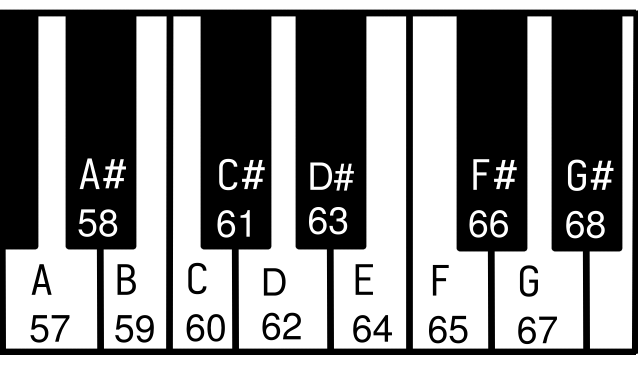
\includegraphics[width=0.3\textwidth]{images/piano/pianoMidi.png}
  \caption{Numérotations MIDI du centre du piano}
  \label{fig:pianoMidi}
\end{figure}
%\end{wrapfigure}

\begin{defi}(Représentaion MIDI d'une note)
  \label{def:MIDI note}
  La représentation MIDI d'une note de musique est définie comme suit.
  Le do central du piano (en général $261.63$Hz) est numéroté à $60$, et le 
  reste des notes est numéroté à $60\pm\alpha$ où $\alpha$ est le décalage au 
  do en nombre de demi ton (négatif si la note est plus basse).
  Ainsi, la valeur midi du la (de $440$Hz) est $69$.
  Dans la figure \ref{fig:pianoMidi}, on représente les numérotations MIDI 
  des notes centrales du piano.
\end{defi}

Nous définissons maintenant ce qu'est un accord.

\begin{defi}(Accord)
  \label{def:Accord}
  Un accord est un ensemble d'ensembles de notes, où chacun des éléments est
  construit en suivant des règles. 
  Il est défini par sa fondamentale (la note de construction) et les
  intervalles, c'est à dire les écarts entre chaque note et la fondamentale.
  Les notes sont définies sans notions d'octaves et l'accord peut donc-être
  renversé ou avec des répétitions (voir \ref{fig:pianoAccords}).
 \end{defi}

Nous choisissons d'encoder les accords de la manière suivante :
$$Acc := (\textbf{fonda}, u_0, \dots, u_n)$$
Où $\textbf{fonda}$ est la note de construction de l'accord, et
$\left\{u_i\right\}_{i\in\llbracket 0,n\rrbracket}$ sont les positions
relatives de chacunes des notes par rapport à $\textbf{fonda}$ dans l'ordre
croissant de taille des intervalles, en suivant la notation "américaine" (voir
annexe \ref{subsec:notaAme}).\\

\begin{exemple}  
  
  \begin{figure}[H]
    \centering
    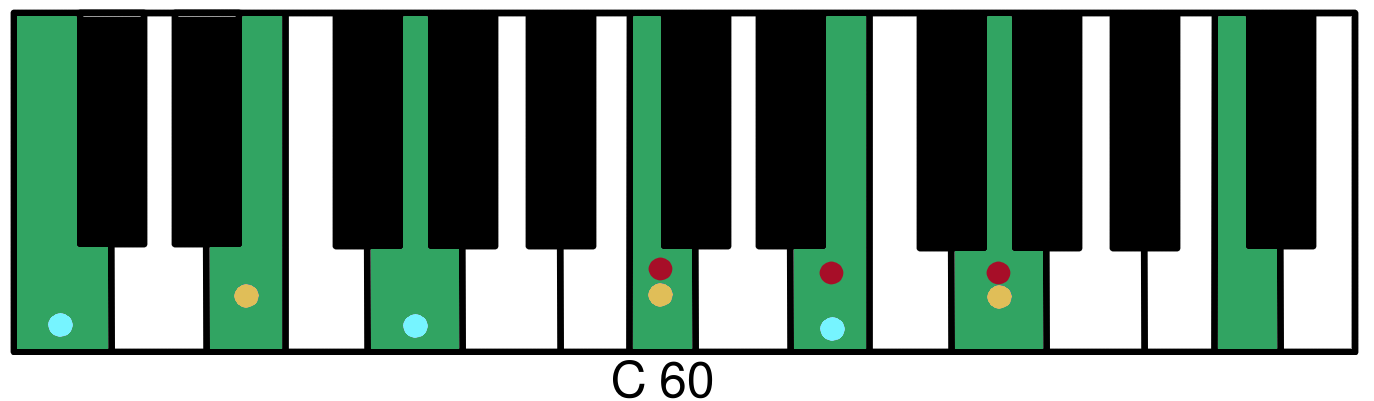
\includegraphics[width=0.6\textwidth]{images/piano/pianoExAccords.png}
    \caption{Trois accords de Do majeur}
    \label{fig:pianoAccords}
  \end{figure}


  La figure \ref{fig:pianoAccords} représente différentes manières de jouer
  l'accord de do majeur (noté $C\texttt{M}$) :
  \begin{itemize}
    \item les notes autorisées sont en vert.
    \item $\left(60, 0, 4, 7\right)$ représenté en rouge.
    \item $\left(60, 0, -8, 7\right)$ représenté en jaune.
    \item $\left(48, 0, 16, 7\right)$ représenté en bleu.
  \end{itemize}
  Les trois accords sont des accords de do majeur. 
  La liste n'est pas exhaustive.
\end{exemple}

\begin{defi}(Guitare)
  \label{def:Guitare}
  On appelera par la suite guitare tout instrument qui possède un manche
  similaire à celui d'une guitare, les variables d'une guitare seront :
  \begin{itemize}
    \item Son nombre de cordes
    \item Sa scordature, (la note de chacune des cordes à vide)
    \item Son nombre de frettes (les petites barres présentes sur le
      manche délimitant les demis tons).
  \end{itemize}
  Pour toutes les guitares, augmenter d'une frette sur une corde augmente d'un 
  demi-ton la note jouée.
\end{defi}


\begin{wrapfigure}{l}{0.4\textwidth}
  \centering \tablature{0.35}{6}{4}{1, -1, 3, 0, 4, 2}
  \caption{
    Exemple de tablature.\\
    Ici, la guitare possède $6$ cordes\\
    et au moins $4$ frettes.
  }
  \label{tabla:Premiere}
\end{wrapfigure}
Pour représenter une position sur le manche de la guitare, on utilise une
tablature. 
Une tablature représente le manche de la guitare et les positions des doigts.
Chaque point représente un point d'appui sur une corde en fonction de la
frette.
On représente comme dans la figure \ref{tabla:Premiere} une position par une 
tablature.\\
Le haut du manche est représenté par une double barre.
Un point bleu représente un point de pression sur le manche (entre deux frettes
sur une corde).
Un point rouge représente une corde non jouée, c'est à dire que l'on ne pince
pas la corde au moment de jouer l'accord.\\
Un point vert représente une corde à vide, c'est une corde pincée au moment de
jouer l'accord, mais sur laquelle on n'exerce pas de pression.
On utilisera cette représentation dans la suite du rapport.


  \begin{figure}[H]
    \centering
    \begin{subfigure}{0.49\textwidth}
      \centering
      \tablature{0.39}{6}{3}{1, 2, 1, 3, 1, 1}
      \caption{Tablature avec barré}
      \label{tabla:Barre}
    \end{subfigure}
    \hfill
    \begin{subfigure}{0.49\textwidth}
      \centering \tablature{0.39}{6}{3}{1,2,1,3,1,0}
      \caption{Tablature avec barré partiel}
      \label{tabla:BarrePartiel}
    \end{subfigure}
    \label{tabla:Double}
    \caption{Tablatures avec barré}
  \end{figure}

Une technique utilisée par les guitaristes est la technique du barré.
Elle consiste a utiliser un doigt pour bloquer toute ou partie des cordes sur
le même niveau.
Par exemple, dans la représentation \ref{tabla:Barre} on remarque que l'on
ne peut pas utiliser $6$ doigts pour bloquer chacune des six cordes mais l'on
peut utiliser l'index pour bloquer toutes les cordes du manche en première
frette et utiliser l'index et l'annulaire pour bloquer les cordes $2$ et $4$.
Celles-ci sont par ailleurs bloquées par l'index en première frette mais cela
n'est pas contradictoire car seul le point de pression le plus éloigné de la 
tête du manche compte.
Cette technique requiert de la part de l'instrumentiste une maîtrise de son
instrument. Elle peut être adaptée de sorte que le barré soit partiel, en ne
commençant pas sur la première ou la dernière corde, ce qui permet de
réaliser une position semblable à la tablature \ref{tabla:BarrePartiel}.


\subsection{Programmation par contraintes}
\label{subsec:CP}

Au cours de ce stage, on a eu une approche utilisant la programmation par
contraintes. Nous donnons ici quelques définitions de base de ce paradigme.
La programmation par contraintes (PPC) est un paradigme de programmation 
permettant de résoudre des problèmes combinatoirement grands.
Dans ce paradigme, on sépare un partie modélisation avec le problème de
satisfaction de contraintes, et une partie résolution, qui va utiliser les
contraintes de problème pour réduire la taille de l'espace des solutions.
Pour les définitions suivantes, on s'inspire de \cite{introPPC}.

\begin{defi}(Modèle)
  \label{def:Model}
  Un modèle est un ensemble fini $\indet = \accolades{\indet_i}_{i\in{I}}$ ($I$ 
  fini) de variables indéterminées à valeurs dans un domaine 
  $\domaine = \accolades{\domaine_i}_{i\in I}$, ainsi qu'un ensemble fini 
  $\contr  = \accolades{\contr_j}_{j\in J}$ ($J$ fini) de contraintes sur les 
  variables. On le note :
  $$\defmodele$$
\end{defi}

\begin{defi}(Solution)
  \label{def:Solution}
  Une solution d'un modèle est une instantiation des variables indéterminées
  dans leurs domaines tels que toutes les contraintes soient respectées.
\end{defi}

\begin{defi}(Solver)
  \label{def:Solver}
  Un solver est un programme qui a pour entrée un modèle \ref{def:Model} et qui
  trouve toutes les solutions, ou une solution particulière \ref{def:Solution} 
  de ce modèle.
  Par la suite on utilisera le solver Choco \cite{Choco} pour modéliser notre
  problème et pour trouver les solutions qui nous intéressent.
\end{defi}

Pour résoudre notre problème, nous allons utiliser la programmation par
contraintes \ref{def:PCC}. Pour ce faire, nous allons créer un modèle (définir
des indéterminées, leurs domaines et des contraintes) dont les 
solutions soients les suites de positions les plus adaptées.
\newpage
